\begin{problem}[1.5]
  In Example 1.8(a) we saw a sequence in $C([0, 1])$ that converges in the $L^1$ metric but not in the sup metric. Prove that the reverse cannot happen: every sequence that converges in the sup metric converges in the $L^1$ metric.
\end{problem}

\begin{solution}
  Let $(f_n)$ be a sequence in $C([0,1])$ and suppose
  \[%
    \metric_\infty(f_n, f) := \sup_{x\in[0, 1]} |f_n(x) - f(x)| \to 0
  ,\]%
  as $n \to \infty$, for some function $f$ in $C([0, 1])$. For each $n$ and every $x\in[0,1]$ we have the pointwise inequality
  \[%
    |f_n(x) - f(x)| \le \metric_\infty(f_n, f)
  .\]%
  Integrating both sides over $[0,1]$ yields
  \[%
    \int_0^1 |f_n(x) - f(x)| \dx \le \int_0^1 \metric_\infty(f_n, f) \dx = \metric_\infty(f_n, f) \cdot 1
  .\]%
  Hence, with $\metric_1(g, h):=\int_0^1 |g(x)-h(x)| \dx$, we get
  \[%
    \metric_1(f_n, f) \le \metric_\infty(f_n, f) \to 0
  .\]%
  Therefore $\metric_1(f_n, f) \to 0$, i.e. $f_n \to f$ in the $L^1$ metric on $C([0,1])$.
\end{solution}

\begin{problem}[1.6]
  Let $(X, \metric)$ be a metric space. Prove the reverse \emph{triangle inequality}:
  \[%
    |\metric(p, q) - \metric(p, r)| \le \metric(q, r)
  ,\]%
  for all $p, q, r \in X$. Include an appropriate picture.
\end{problem}

\begin{solution}
  Let $p,q,r \in X$. By the triangle inequality we have
  \[%
    \metric(p, q) \le \metric(p, r) + \metric(r, q)
  ,\]%
  which can be rewritten as
  \[%
    \metric(p, q) - \metric(p, r) \le \metric(r, q) = \metric(q, r)
  .\]%
  Similarly, swapping $q$ and $r$ gives
  \[%
    \metric(p, r) \le \metric(p, q) + \metric(q, r) \implies \metric(p, r) - \metric(p, q) \le \metric(q, r)
  ,\]%
  or equivalently
  \[%
    -\metric(q, r) \le \metric(p, q) - \metric(p, r)
  .\]%
  Combining these two inequalities yields the reverse triangle inequality:
  \[%
    |\metric(p, q) - \metric(p, r)| \le \metric(q, r)
  .\]%

  \begin{figure}[H]
    \centering
    \begin{tikzpicture}[scale=2]
      % Points
      \coordinate (P) at (0,0);
      \coordinate (Q) at (2,1);
      \coordinate (R) at (1,2);

      % Triangle
      \draw[thick] (P) -- (Q) -- (R) -- cycle;

      % Points labels
      \filldraw[black] (P) circle (0.03) node[below left] {$p$};
      \filldraw[black] (Q) circle (0.03) node[below right] {$q$};
      \filldraw[black] (R) circle (0.03) node[above] {$r$};

      % Distance labels
      \node at ($(P)!0.5!(Q)$) [below, yshift=-3pt, xshift=3pt] {$\metric(p, q)$};
      \node at ($(P)!0.5!(R)$) [left] {$\metric(p, r)$};
      \node at ($(Q)!0.5!(R)$) [right] {$\metric(q, r)$};
    \end{tikzpicture}
    \caption{Visualization of the reverse triangle inequality in a metric space.}\vspace{-\dp\strutbox}\vspace{-\dp\strutbox}\vspace{-\dp\strutbox}\vspace{-\dp\strutbox}\vspace{-\dp\strutbox}\vspace{-\dp\strutbox}\vspace{-\dp\strutbox}
  \end{figure}
\end{solution}

\begin{problem}[1.7]
  Let $(X, \metric_X)$ and $(Y, \metric_Y)$ and $(Z, \metric_Z)$ be metric spaces. Let $f : X \to Y$ be continuous at a point $p \in X$, and let $g : Y \to Z$ be continuous at $f(p)$. Prove that $g \circ f$ is continuous at $p$.
\end{problem}

\begin{solution}
  Let $(X, \metric_X)$, $(Y, \metric_Y)$ and $(Z, \metric_Z)$ be metric spaces, let $f : X \to Y$ be continuous at $p \in X$, and let $g : Y \to Z$ be continuous at $f(p)$. We show $g \circ f$ is continuous at $p$.

  Fix $\epsilon > 0$. Since $g$ is continuous at $f(p)$, there exists $\delta_2 > 0$ such that
  \[%
    \metric_Y(y, f(p)) < \delta_2 \implies \metric_Z(g(y), g(f(p))) < \epsilon
  .\]%
  Since $f$ is continuous at $p$, there exists $\delta_1 > 0$ such that
  \[%
    \metric_X(x, p) < \delta_1 \implies \metric_Y(f(x), f(p)) < \delta_2
  .\]%
  Now let $x \in X$ satisfy $\metric_X(x, p) < \delta_1$. Then by the previous implication $\metric_Y(f(x), f(p)) < \delta_2$, and therefore by the choice of $\delta_2$ we have $\metric_Z(g(f(x)), g(f(p))) < \epsilon$. This shows that for every $\epsilon > 0$, take $\delta = \delta_1$ to get
  \[%
    \metric_X(x, p) < \delta \implies \metric_Z(g(f(x)), g(f(p))) < \epsilon
  .\]%
  Therefore, $g \circ f$ is continuous at $p$.
\end{solution}

\begin{problem}[2.1]
  Sketch each subset of $\R^2$ and find its closure, interior, and boundary in the Euclidean metric:
  \begin{enumerate}
    \item $A_1 = \{(x, y) \mid 0 < x \le 1, 0 \le y < 1\}$.
    \item $A_2 = \{(x, y) \mid 0 < x \le 1, y = 0\}$.
    \item $A_3 = \{(x, y) \mid x \in \Q~\text{or}~y \in \Q\}$.
    \item $A_4 = \{(x, y) \mid x \ne 0~\text{or}~y = 0\}$.
  \end{enumerate}
\end{problem}

\begin{solution}[(i)]
  The boundary of $A_1$ is the rectangle formed by the lines $x = 0$, $x = 1$, $y = 0$, and $y = 1$. The interior is the open rectangle bounded by those same lines, and the closure is the union of the interior and the boundary, that is, the closed rectangle $[0,1] \times [0,1]$.
  \begin{figure}[H]
    \centering

    % Interior
    \begin{subfigure}[b]{0.3\textwidth}
      \centering
      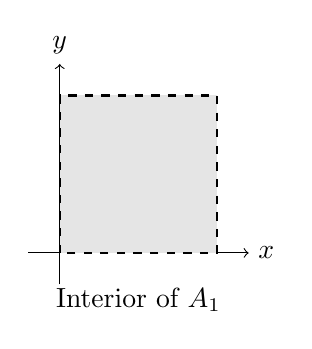
\begin{tikzpicture}[scale=2]
        % Axes
        \draw[->] (-0.2,0) -- (1.2,0) node[right] {$x$};
        \draw[->] (0,-0.2) -- (0,1.2) node[above] {$y$};

        % Interior (open rectangle)
        \filldraw[fill=gray!20, draw=none] (0,0) rectangle (1,1);
        % Hollow boundary (to show open)
        \draw[dashed, thick] (0,0) rectangle (1,1);

        % Labels
        \node at (0.5,-0.3) {Interior of $A_1$};
      \end{tikzpicture}
    \end{subfigure}
    \hfill
    % Boundary
    \begin{subfigure}[b]{0.3\textwidth}
      \centering
      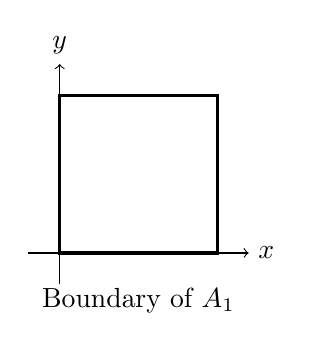
\begin{tikzpicture}[scale=2]
        % Axes
        \draw[->] (-0.2,0) -- (1.2,0) node[right] {$x$};
        \draw[->] (0,-0.2) -- (0,1.2) node[above] {$y$};

        % Boundary (solid square)
        \draw[very thick, black] (0,0) rectangle (1,1);

        % Labels
        \node at (0.5,-0.3) {Boundary of $A_1$};
      \end{tikzpicture}
    \end{subfigure}
    \hfill
    % Closure
    \begin{subfigure}[b]{0.3\textwidth}
      \centering
      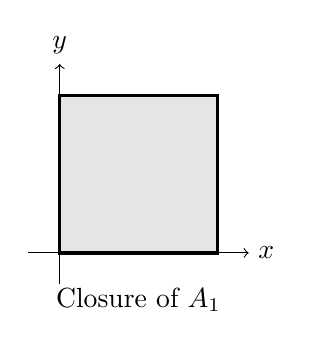
\begin{tikzpicture}[scale=2]
        % Axes
        \draw[->] (-0.2,0) -- (1.2,0) node[right] {$x$};
        \draw[->] (0,-0.2) -- (0,1.2) node[above] {$y$};

        % Closure (filled + boundary)
        \filldraw[fill=gray!20, draw=black, very thick] (0,0) rectangle (1,1);

        % Labels
        \node at (0.5,-0.3) {Closure of $A_1$};
      \end{tikzpicture}
    \end{subfigure}

    \caption{Visualization of the interior, boundary, and closure of $A_1 = [0,1] \times [0,1]$.}\vspace{-\dp\strutbox}\vspace{-\dp\strutbox}\vspace{-\dp\strutbox}\vspace{-\dp\strutbox}\vspace{-\dp\strutbox}\vspace{-\dp\strutbox}\vspace{-\dp\strutbox}
  \end{figure}
\end{solution}

\begin{solution}[(ii)]
  The set $A_2 = \{(x, y) \mid 0 < x \le 1,\, y = 0\}$ is a half-open line segment on the $x$-axis. Its interior is empty, since it has no open neighborhood contained in $A_2$. Its boundary is the closed segment $[0,1] \times \{0\}$, and its closure is that same closed segment.

  \begin{figure}[H]
    \centering

    % Interior
    \begin{subfigure}[b]{0.3\textwidth}
      \centering
      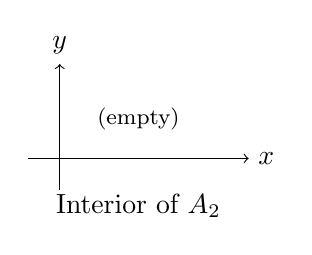
\begin{tikzpicture}[scale=2]
        \draw[->] (-0.2,0) -- (1.2,0) node[right] {$x$};
        \draw[->] (0,-0.2) -- (0,0.6) node[above] {$y$};

        % Empty interior
        \node at (0.5,0.25) {\footnotesize (empty)};

        \node at (0.5,-0.3) {Interior of $A_2$};
      \end{tikzpicture}
    \end{subfigure}
    \hfill
    % Boundary
    \begin{subfigure}[b]{0.3\textwidth}
      \centering
      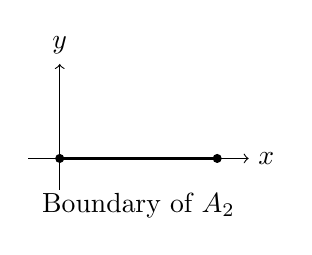
\begin{tikzpicture}[scale=2]
        \draw[->] (-0.2,0) -- (1.2,0) node[right] {$x$};
        \draw[->] (0,-0.2) -- (0,0.6) node[above] {$y$};

        % Boundary segment [0,1] × {0}
        \draw[very thick, black] (0,0) -- (1,0);
        \filldraw[black] (0,0) circle (0.025);
        \filldraw[black] (1,0) circle (0.025);

        \node at (0.5,-0.3) {Boundary of $A_2$};
      \end{tikzpicture}
    \end{subfigure}
    \hfill
    % Closure
    \begin{subfigure}[b]{0.3\textwidth}
      \centering
      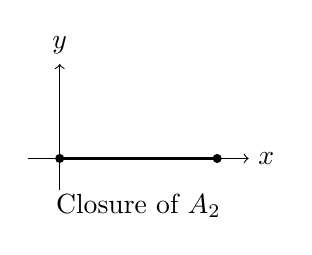
\begin{tikzpicture}[scale=2]
        \draw[->] (-0.2,0) -- (1.2,0) node[right] {$x$};
        \draw[->] (0,-0.2) -- (0,0.6) node[above] {$y$};

        % Closure [0,1] × {0}
        \draw[very thick, black] (0,0) -- (1,0);
        \filldraw[black] (0,0) circle (0.025);
        \filldraw[black] (1,0) circle (0.025);

        \node at (0.5,-0.3) {Closure of $A_2$};
      \end{tikzpicture}
    \end{subfigure}

    \caption{Visualization of the interior, boundary, and closure of $A_2 = \{(x, y) \mid 0 < x \le 1,\, y = 0\}$.}\vspace{-\dp\strutbox}\vspace{-\dp\strutbox}\vspace{-\dp\strutbox}\vspace{-\dp\strutbox}\vspace{-\dp\strutbox}\vspace{-\dp\strutbox}\vspace{-\dp\strutbox}
  \end{figure}
\end{solution}

\begin{solution}[(iii)]
  The set $A_3 = \{(x, y) \mid x \in \Q~\text{or}~y \in \Q\}$ is dense in $\R^2$, since every open ball contains points with rational coordinates. However, its interior is empty because any open set in $\R^2$ also contains points whose $x$ and $y$ coordinates are both irrational. Therefore, its boundary and closure are both equal to $\R^2$.

  \begin{figure}[H]
    \centering

    % Interior
    \begin{subfigure}[b]{0.3\textwidth}
      \centering
      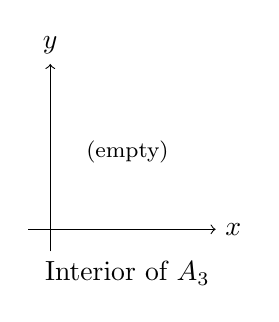
\begin{tikzpicture}[scale=1.4]
        \draw[->] (-0.2,0) -- (1.5,0) node[right] {$x$};
        \draw[->] (0,-0.2) -- (0,1.5) node[above] {$y$};

        \node at (0.7,0.7) {\footnotesize (empty)};
        \node at (0.7,-0.4) {Interior of $A_3$};
      \end{tikzpicture}
    \end{subfigure}
    \hfill
    % Boundary
    \begin{subfigure}[b]{0.3\textwidth}
      \centering
      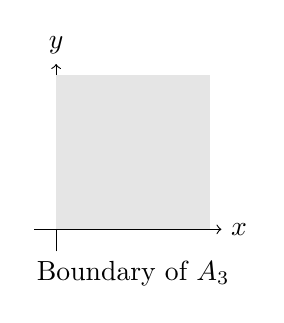
\begin{tikzpicture}[scale=1.4]
        \draw[->] (-0.2,0) -- (1.5,0) node[right] {$x$};
        \draw[->] (0,-0.2) -- (0,1.5) node[above] {$y$};

        \fill[gray!20] (0,0) rectangle (1.4,1.4);

        \node at (0.7,-0.4) {Boundary of $A_3$};
      \end{tikzpicture}
    \end{subfigure}
    \hfill
    % Closure
    \begin{subfigure}[b]{0.3\textwidth}
      \centering
      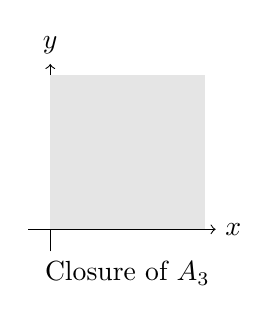
\begin{tikzpicture}[scale=1.4]
        \draw[->] (-0.2,0) -- (1.5,0) node[right] {$x$};
        \draw[->] (0,-0.2) -- (0,1.5) node[above] {$y$};

        \fill[gray!20] (0,0) rectangle (1.4,1.4);

        \node at (0.7,-0.4) {Closure of $A_3$};
      \end{tikzpicture}
    \end{subfigure}

    \caption{Visualization of the interior, boundary, and closure of $A_3 = \{(x, y) \mid x \in \Q~\text{or}~y \in \Q\}$.}\vspace{-\dp\strutbox}\vspace{-\dp\strutbox}\vspace{-\dp\strutbox}\vspace{-\dp\strutbox}\vspace{-\dp\strutbox}\vspace{-\dp\strutbox}\vspace{-\dp\strutbox}
  \end{figure}
\end{solution}

\begin{solution}[(iv)]
  The set $A_4 = \{(x, y) \mid x \ne 0~\text{or}~y = 0\}$ is the entire plane except for the $y$-axis, with the $x$-axis added back in. Its interior is $A_4$ itself, since removing a one-dimensional subset from $\R^2$ does not affect openness. The boundary consists of the $y$-axis, and the closure is the whole plane $\R^2$.

  \begin{figure}[H]
    \centering

    % Interior
    \begin{subfigure}[b]{0.3\textwidth}
      \centering
      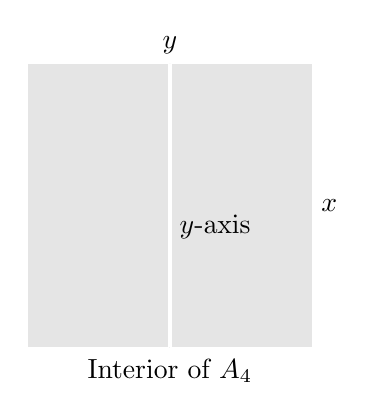
\begin{tikzpicture}[scale=1.5]
        \draw[->] (-1.2,0) -- (1.2,0) node[right] {$x$};
        \draw[->] (0,-1.2) -- (0,1.2) node[above] {$y$};

        % Shade plane except y-axis
        \fill[gray!20] (-1.2,-1.2) rectangle (1.2,1.2);
        \fill[white] (-0.02,-1.2) rectangle (0.02,1.2);

        \node at (0,0) [below right] {$y$-axis};
        \node at (0,-1.4) {Interior of $A_4$};
      \end{tikzpicture}
    \end{subfigure}
    \hfill
    % Boundary
    \begin{subfigure}[b]{0.3\textwidth}
      \centering
      \begin{tikzpicture}[scale=1.5]
        \draw[->] (-1.2,0) -- (1.2,0) node[right] {$x$};
        \draw[->] (0,-1.2) -- (0,1.2) node[above] {$y$};

        % y-axis (boundary)
        \draw[very thick, black] (0,-1.2) -- (0,1.2);

        \node at (0.6,-1.4) {Boundary of $A_4$};
      \end{tikzpicture}
    \end{subfigure}
    \hfill
    % Closure
    \begin{subfigure}[b]{0.3\textwidth}
      \centering
      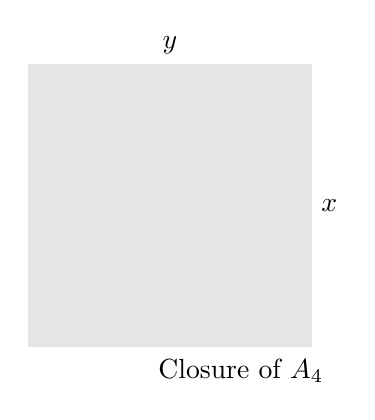
\begin{tikzpicture}[scale=1.5]
        \draw[->] (-1.2,0) -- (1.2,0) node[right] {$x$};
        \draw[->] (0,-1.2) -- (0,1.2) node[above] {$y$};

        % Whole plane shaded
        \fill[gray!20] (-1.2,-1.2) rectangle (1.2,1.2);

        \node at (0.6,-1.4) {Closure of $A_4$};
      \end{tikzpicture}
    \end{subfigure}

    \caption{Visualization of the interior, boundary, and closure of $A_4 = \{(x, y) \mid x \ne 0~\text{or}~y = 0\}$.}\vspace{-\dp\strutbox}\vspace{-\dp\strutbox}\vspace{-\dp\strutbox}\vspace{-\dp\strutbox}\vspace{-\dp\strutbox}\vspace{-\dp\strutbox}\vspace{-\dp\strutbox}
  \end{figure}
\end{solution}

\begin{problem}[2.3]
  Let $(X, \metric)$ be a metric space and $A \subset X$. Use Proposition 2.6 to prove that
  \[%
    \partial A = \partial(X \setminus A) = \overline A \cap \overline{X \setminus A}
  .\]%
\end{problem}

\begin{solution}
  Assume $x \in \partial A$. By definition, that means $x \in \overline A \setminus \sint A$. Then, $x \in \overline A$ and $x \notin \sint A$. By Proposition~2.6, we have $x \notin \sint A$ if and only if $x \in \overline{X \setminus A}$. Therefore, $x \in \overline A$ and $x \in \overline{X \setminus A}$, which implies
  \[%
    x \in \overline A \cap \overline{X \setminus A}
  .\]%
  Hence, $\partial A \subset \overline A \cap \overline{X \setminus A}$.

  Now, for the converse. Assume $x \in \overline A \cap \overline{X \setminus A}$. Then, $x \in \overline A$ and $x \in \overline{X \setminus A}$. By Proposition~2.6 again, $x \in \overline{X \setminus A}$ if and only if $x \notin \sint A$. Therefore, $x \in \overline A$ and $x \notin \sint A$, which means $x \in \partial A$. Hence,
  \[%
    \overline A \cap \overline{X \setminus A} \subset \partial A
  .\]%

  Combining both inclusions, we conclude that
  \[%
    \partial A = \overline A \cap \overline{X \setminus A}
  .\]%
  Finally, since the expression is symmetric in $A$ and $X \setminus A$, it follows that
  \[%
    \partial A = \partial(X \setminus A)
  .\qedhere\]%
\end{solution}

\begin{problem}[2.6]
  We saw in Example 2.8 that the inclusion $\sint A \cup \sint B \subset \sint(A \cup B)$ can be strict. Prove however that if $\overline A \cap \overline B = \emptyset$ then $\sint A \cup \sint B = \sint(A \cup B)$.
\end{problem}

\begin{solution}
  We always have
  \[%
    \sint A \cup \sint B \subset \sint(A\cup B)
  ,\]%
  so it remains to prove the reverse inclusion under the assumption
  \[%
    \overline A \cap \overline B = \emptyset
  .\]%

  Let $x \in \sint(A \cup B)$. Then there exists an open neighbourhood $U$ of $x$ with $U \subset A\cup B$. We will show that $x \in \sint A$ or $x \in \sint B$.

  Suppose, for contradiction, that $x \notin \sint A$ and $x \notin \sint B$. Since $x \notin \sint A$, every neighbourhood of $x$ meets the complement $X \setminus A$. In particular $U$ meets $X \setminus A$. But $U \subset A \cup B$, so any point of $U \cap (X \setminus A)$ must lie in $B$. Hence $U \cap B \neq \emptyset$, and because this holds for every neighbourhood of $x$ we conclude $x \in\overline B$. By the same argument (swapping $A$ and $B$) the assumption $x \notin\sint B$ implies $x \in\overline A$. Thus
  \[%
    x \in\overline A \cap\overline B
  ,\]%
  contradicting the hypothesis that $\overline A \cap \overline B = \emptyset$.

  Therefore at least one of $x \in\sint A$ or $x \in\sint B$ must hold, so
  \[%
    x \in\sint A \cup \sint B
  .\]%
  This proves $\sint(A \cup B) \subset \sint A \cup \sint B$, and combined with the trivial inclusion we obtain
  \[%
    \sint(A \cup B) = \sint A \cup \sint B
  .\qedhere\]%
\end{solution}
